
    \documentclass[a4paper,12pt]{article}
    \usepackage[utf8]{inputenc}
    \usepackage{graphicx}
    \usepackage{multicol}
    \usepackage{fancyhdr}
    \usepackage[paperwidth=210mm, paperheight=210mm, margin=25mm]{geometry}
    \usepackage{xcolor}
    \usepackage{hyperref}

    \definecolor{triton_green}{RGB}{4,106,56}
    \definecolor{A}{RGB}{129, 213, 82}
    \definecolor{B}{RGB}{249, 217, 87}
    \definecolor{C}{RGB}{226, 121, 46}
    \definecolor{D}{RGB}{220, 59, 38}

    % \setlength{\fboxsep}{0pt}

    % Set up header and footer
    \pagestyle{fancy}
    \fancyhf{}
    \fancyhead[L]{Gobar NCRAP}
    \fancyhead[C]{}
    \fancyhead[R]{\textit{bit.ly/gobarncrap}}
    \renewcommand{\headrulewidth}{0.5pt}

    % Reduce the space between columns
    \setlength{\columnsep}{10pt}  % Adjust the value to reduce the gap

    % Document begins
    \begin{document}

    % Title
    \begin{center}
        {\color{triton_green} \Large \textbf{Honda BALLADE earns C grade}}\\
        \vspace{0.5cm}
        {\large \textit{New release of seatbelt reminder results from Gobar NCRAP!}}
    \end{center}

    % Begin multicolumn layout
    \begin{multicols}{2}

    % First column content
    Today, Gobar NCRAP is releasing the seatbelt reminder grades for the Honda BALLADE.\\

    The \textbf{Honda BALLADE} earns a \colorbox{C}{\textbf{C}} grade. It activates its rear seatbelt reminder visual signal when any rear seatbelt is not fastened. It activates its acoustic signal when any rear seatbelt changes its status to 'unfastened'. 

    \begin{center}
        \noindent \fbox{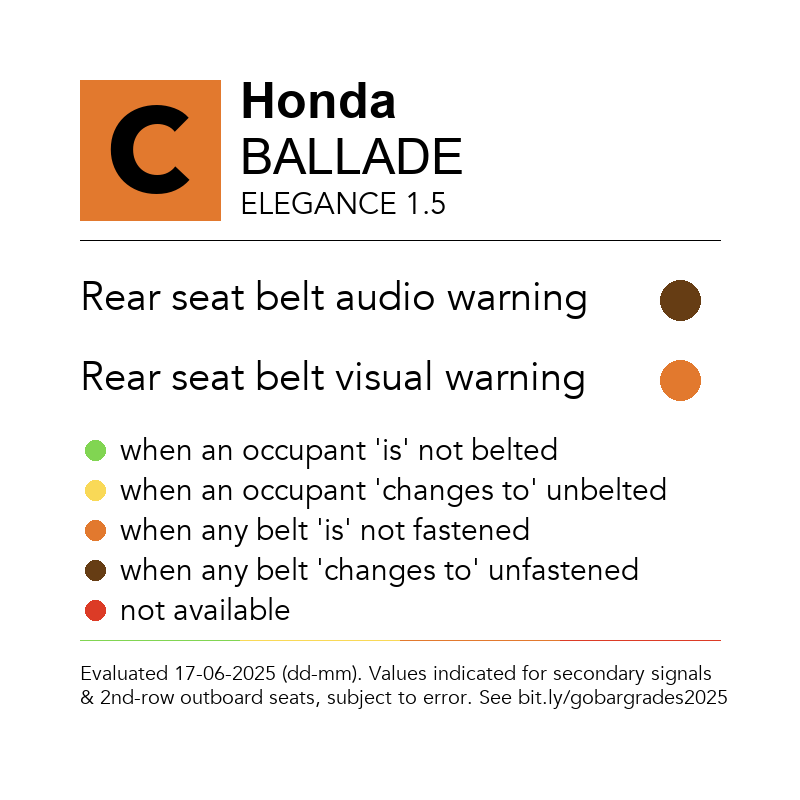
\includegraphics[width=0.95\linewidth]{17-06-2025/scorecard.png}}
    \end{center}
                               
    \begin{center}
        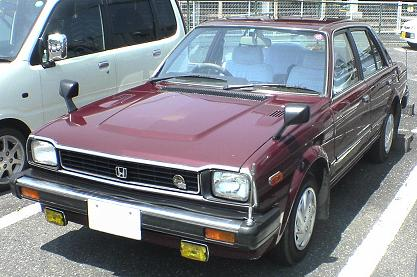
\includegraphics[width=0.95\linewidth]{17-06-2025/model.png}
        \textit{The Honda BALLADE (image: Wikimedia)}
    \end{center}

    \begin{footnotesize}
        \vspace{0.02in}\hrule\vspace{0.02in}\noindent Gobar NCRAP is an independent, noncommercial blog that evaluates the safety specification of vehicles sold to Indian consumers. The 2025 Gobar Grades assign letter grades -- A, B, C or D -- to vehicle models based on the behaviour of their rear seatbelt reminders. The evaluation criteria reward the fitment of intelligent reminders with occupant detection in all rear seats, as opposed to the less effective change-of-status alerts or permanent warnings accepted by upcoming regulations and given full credit by existing consumer test programmes targeting the Indian vehicle market. Detailed evaluation criteria are available at: \href{https://gobarncrap.wixsite.com/gobar-ncrap/about}{gobarncrap.wixsite.com/gobar-ncrap/about} The latest details of individual grades are at the following URL: \href{https://gobarncrap.wixsite.com/gobar-ncrap/2025-evaluations}{bit.ly/gobargrades2025}.
        \vspace{0.02in}\hrule
    \end{footnotesize}
    \end{multicols}
    
    \end{document}
    